\documentclass[12pt]{article}

% Modelo oficial SBC, versão disponibilizada no template v2017.
% sbc-template.sty e sbc.bst são cópias literais dos arquivos fornecidos.
\usepackage{sbc-template}
% Compatibilidade sem editar o estilo oficial: o hook v2017 omite o ramo
% falso de \@ifpackageloaded{hyperref}. O token neutro evita consumir
% o primeiro comando do próximo hook (por exemplo, o do babel).
\AddToHook{begindocument/before}[sbc-template]{\relax}
\usepackage[T1]{fontenc}
\usepackage[utf8]{inputenc}
\usepackage[english,brazilian]{babel}
\usepackage{graphicx,url}
\usepackage{amsmath,amssymb}
\usepackage{booktabs}
\usepackage{algorithm}
\usepackage{algpseudocode}
\usepackage{listings}
\usepackage{placeins}
\usepackage[hidelinks]{hyperref}

\sloppy
\graphicspath{{figures/}}
\addto\captionsbrazilian{\renewcommand{\refname}{Referências Bibliográficas}}
\floatname{algorithm}{Algoritmo}
\captionsetup[algorithm]{font={sf,bf,footnotesize},labelsep=period}
\algrenewcommand{\algorithmicrequire}{\textbf{Entrada:}}
\algrenewcommand{\algorithmicensure}{\textbf{Saída:}}
\algrenewcommand{\algorithmicif}{\textbf{se}}
\algrenewcommand{\algorithmicthen}{\textbf{então}}
\algrenewcommand{\algorithmicelse}{\textbf{senão}}
\algrenewcommand{\algorithmicfor}{\textbf{para}}
\algrenewcommand{\algorithmicwhile}{\textbf{enquanto}}
\algrenewcommand{\algorithmicdo}{\textbf{faça}}
\algrenewcommand{\algorithmicend}{\textbf{fim}}
\algrenewcommand{\algorithmicreturn}{\textbf{retornar}}
\newcommand{\OPT}{\operatorname{OPT}}

\lstdefinestyle{java}{
  language=Java,
  basicstyle=\ttfamily\fontsize{8}{9.5}\selectfont,
  numbers=left,
  numberstyle=\tiny,
  numbersep=6pt,
  xleftmargin=1.8em,
  frame=lines,
  breaklines=true,
  breakatwhitespace=false,
  columns=fullflexible,
  keepspaces=true,
  showstringspaces=false,
  tabsize=4,
  captionpos=t,
  inputencoding=utf8,
  extendedchars=true,
  literate=
    {á}{{\'a}}1 {à}{{\`a}}1 {â}{{\^a}}1 {ã}{{\~a}}1
    {é}{{\'e}}1 {ê}{{\^e}}1 {í}{{\'i}}1
    {ó}{{\'o}}1 {ô}{{\^o}}1 {õ}{{\~o}}1 {ú}{{\'u}}1 {ü}{{\"u}}1 {ç}{{\c c}}1
    {Á}{{\'A}}1 {À}{{\`A}}1 {Â}{{\^A}}1 {Ã}{{\~A}}1
    {É}{{\'E}}1 {Ê}{{\^E}}1 {Í}{{\'I}}1
    {Ó}{{\'O}}1 {Ô}{{\^O}}1 {Õ}{{\~O}}1 {Ú}{{\'U}}1 {Ü}{{\"U}}1 {Ç}{{\c C}}1
    {º}{{\textordmasculine}}1 {ª}{{\textordfeminine}}1
    {—}{{---}}1 {–}{{--}}1 {→}{{$\to$}}1 {≤}{{$\leq$}}1 {≥}{{$\geq$}}1
}
\lstset{style=java}
\renewcommand{\lstlistingname}{Listagem}
% Gerado dos CSVs reais por ReportStats.java.
% Gerado por ferramentas/ReportStats.java; não editar valores manualmente.
\newcommand{\TotalInstances}{230}
\newcommand{\RandomInstances}{200}
\newcommand{\StructuredInstances}{30}
\newcommand{\OptimalInstances}{228}
\newcommand{\TimeoutInstances}{2}
\newcommand{\RawMeasurements}{690}
\newcommand{\RawTimeouts}{6}
\newcommand{\QualityInstances}{223}
\newcommand{\ZeroInstances}{5}
\newcommand{\FasterApproxInstances}{230}
\newcommand{\EqualPositiveInstances}{2}
\newcommand{\EqualTotalInstances}{7}
\newcommand{\FactorTwoInstances}{47}
\newcommand{\MeanRatio}{1,493}
\newcommand{\MedianRatio}{1,400}
\newcommand{\MeanGap}{49,30}
\newcommand{\RandomMeanRatio}{1,453}
\newcommand{\StructuredMeanRatio}{1,823}


\title{Uma Análise Experimental de Algoritmos para o\\
Problema da Cobertura Mínima por Vértices}

% Iniciais intermediárias mantêm os três autores na linha prevista pelo SBC.
% Nomes completos constam dos metadados do PDF e do README do projeto LaTeX.
\author{Ian P. P. Bomfim\inst{1}, João M. A. Constâncio\inst{1}, Ramon V. S. Corrêa\inst{1}}
\address{Pontifícia Universidade Católica de Minas Gerais (PUC Minas)\\
  Projeto e Análise de Algoritmos -- Trabalho Prático 2\\
  Professor: Walisson Ferreira de Carvalho}

\hypersetup{
  pdftitle={Uma Análise Experimental de Algoritmos para o Problema da Cobertura Mínima por Vértices},
  pdfauthor={Ian Pereira Pinto Bomfim; João Miguel de Abreu Constâncio; Ramon Vinícius Silva Corrêa},
  pdfsubject={Projeto e Análise de Algoritmos -- Java 17 puro -- Vertex Cover},
  pdfkeywords={vertex cover, branch and bound, maximal matching, approximation algorithms}
}

\begin{document}
\maketitle

\begin{otherlanguage}{english}
\begin{abstract}
This paper compares a branch-and-bound solver and a maximal-matching
2-approximation for minimum vertex cover, implemented in plain Java 17.
The study uses 230 graphs and three measurements per algorithm and instance.
The exact solver certifies 228 optima; two instances reach the time limit.
Among 223 instances with a proven positive optimum, the mean approximation
ratio is 1.493. The approximation is faster in all selected measurements.
The analysis distinguishes feasible solutions from proven optima and discusses
the limits of the experimental evidence.
\end{abstract}
\end{otherlanguage}

\begin{resumo}
Este trabalho compara Branch and Bound e uma aproximação por emparelhamento
maximal para Cobertura Mínima por Vértices, implementados em Java 17 puro.
Foram utilizados 230 grafos e três medições por algoritmo e instância.
O exato comprovou 228 ótimos, com dois timeouts no resumo.
Nas 223 instâncias com ótimo comprovado e positivo, a razão média da
aproximação foi 1,493. A aproximação foi mais rápida em todas as medições
selecionadas. A análise distingue soluções válidas de ótimos comprovados
e explicita as limitações da evidência experimental.
\end{resumo}

\section{Introdução}
\label{sec:introduction}

Problemas de otimização combinatória surgem quando é necessário escolher,
entre alternativas discretas, uma solução de menor custo que satisfaça
determinadas restrições. A quantidade de alternativas pode crescer
exponencialmente com a entrada. Nesses casos, a escolha de uma estratégia
algorítmica não envolve apenas obter uma solução: é preciso considerar
o tempo disponível, a qualidade exigida e a possibilidade de demonstrar
que não existe solução melhor \cite{cormen2022,fomin2010}.

O Problema da Cobertura Mínima por Vértices, ou \emph{Minimum Vertex Cover},
expressa essa tensão de forma particularmente clara. Dado um grafo, deseja-se
selecionar o menor conjunto de vértices que contenha pelo menos uma
extremidade de cada aresta. Essa condição permite modelar, sob hipóteses
apropriadas, a seleção de pontos para observar conexões, inspecionar
ligações de uma infraestrutura ou instrumentar relações entre componentes.
A versão de decisão é NP-completa, enquanto a versão de otimização é
NP-difícil \cite{karp1972,garey1979}.

A dificuldade no pior caso não impede estudar algoritmos exatos úteis em
instâncias limitadas. A técnica Branch and Bound organiza uma busca e
elimina ramos quando limites demonstram que eles não podem melhorar a
solução conhecida. Em contraste, algoritmos aproximados podem obter
rapidamente uma cobertura válida com uma garantia matemática sobre sua
cardinalidade. O método por emparelhamento maximal oferece garantia de
fator~2 \cite{cormen2022,vazirani2001}. São propostas com compromissos
distintos, cuja comparação exige não confundir uma boa solução com uma
prova de otimalidade.

O objetivo geral deste trabalho é analisar experimentalmente um Branch
and Bound e uma aproximação por emparelhamento maximal, implementados
em Java~17 puro, comparando tempo, qualidade das coberturas e esforço de
busca em grafos de diferentes tamanhos e densidades. Os objetivos
específicos são formalizar o problema e sua classificação; descrever e
validar os dois algoritmos; gerar instâncias reproduzíveis; medir seu
comportamento sob um limite de tempo; e discutir as vantagens e
limitações sustentadas pelos dados.

A Seção~\ref{sec:theory} apresenta os fundamentos, a demonstração de
NP-Completude e outras abordagens. A Seção~\ref{sec:methodology} descreve
a implementação, os testes e o protocolo. As Seções~\ref{sec:results}
e~\ref{sec:analysis} apresentam e analisam os resultados, respectivamente.
A Seção~\ref{sec:conclusion} sintetiza as conclusões. Os anexos incluem
o código-fonte essencial e instruções de reprodução.

\section{Fundamentação Teórica}
\label{sec:theory}

\subsection{Grafos, emparelhamentos e cobertura por vértices}

Um grafo não direcionado $G=(V,E)$ possui um conjunto de vértices $V$ e um
conjunto de arestas $E$, em que cada aresta é um par não ordenado de
vértices. Neste trabalho, os grafos são simples: não há laços nem arestas
paralelas. O grau $d_G(v)$ é a quantidade de arestas incidentes em $v$;
um vértice de grau zero é isolado. Um grafo completo $K_n$ conecta todos
os pares distintos. Um grafo bipartido admite uma partição
$V=A\mathbin{\dot\cup}B$ sem arestas internas às partes; no bipartido
completo $K_{a,b}$ existem todas as $ab$ arestas entre elas
\cite{cormen2022}.

Um emparelhamento (\emph{matching}) $M\subseteq E$ é um conjunto de arestas
que não compartilham extremos. Ele é \emph{maximal} quando nenhuma aresta
adicional pode ser incluída mantendo essa propriedade. Isso difere de
um emparelhamento \emph{máximo}, que possui a maior cardinalidade entre
todos os emparelhamentos do grafo. A maximalidade é suficiente para a
aproximação implementada, embora não implique cardinalidade máxima
\cite{vazirani2001}.

Uma cobertura por vértices é um conjunto $C\subseteq V$ tal que
\begin{equation}
  \forall\,\{u,v\}\in E,\qquad u\in C\ \lor\ v\in C .
  \label{eq:cover}
\end{equation}
O objetivo da otimização é
\begin{equation}
  \OPT(G)=\min\bigl\{|C|:\ C\subseteq V
       \text{ satisfaz a Equação~\eqref{eq:cover}}\bigr\}.
  \label{eq:opt}
\end{equation}
Uma cobertura \emph{válida} satisfaz a condição de cobertura; uma cobertura
\emph{mínima} atinge o valor da Equação~\eqref{eq:opt}.
Já a \emph{melhor conhecida} é apenas a
menor cobertura válida encontrada durante uma busca. Ela só pode ser
declarada ótima quando há uma demonstração de que nenhuma cobertura menor
existe. Além disso, \emph{mínima} não significa apenas \emph{minimal}:
não conseguir remover individualmente um vértice de uma cobertura não
prova que sua cardinalidade é a menor possível.

\subsection{Classes de complexidade e NP-Completude}

As classes P e NP dizem respeito a problemas de decisão. P reúne os
problemas decididos em tempo polinomial por um algoritmo determinístico.
NP reúne os problemas cujas instâncias positivas possuem certificados de
tamanho polinomial verificáveis em tempo polinomial. Portanto, pertencer
a NP não significa, por si só, ser NP-completo \cite{garey1979,cormen2022}.

Uma redução polinomial $A\leq_p B$ transforma cada instância de $A$ em uma
instância de $B$, em tempo polinomial, preservando a resposta.
Um problema é NP-difícil quando todo problema de NP se reduz a ele.
Um problema de decisão é NP-completo quando, simultaneamente, pertence
a NP e é NP-difícil. A igualdade P=NP permanece em aberto; assim,
NP-Completude não autoriza afirmar que foi provada a inexistência de
algoritmos polinomiais \cite{garey1979}.

Para Vertex Cover de decisão, a entrada é $(G,k)$ e a pergunta é se existe
uma cobertura $C$ com $|C|\leq k$. Dado um conjunto candidato,
verificam-se seus índices, sua cardinalidade e as extremidades de todas
as arestas. Com marcações por vértice, essa verificação custa
$O(|V|+|E|)$, demonstrando o pertencimento a NP.

Para a NP-dificuldade, utiliza-se \emph{Independent Set}, problema de
decisão clássico NP-completo \cite{garey1979}. Dada a instância $(G,k)$,
com $0\leq k\leq |V|$, constrói-se a instância $(G,k')$ de Vertex Cover,
no mesmo grafo, em que
\begin{equation}
  k'=|V|-k,\qquad
  S\text{ é independente em }G
  \ \Longleftrightarrow\
  V\setminus S\text{ é cobertura de }G .
  \label{eq:reduction}
\end{equation}

Para provar o primeiro sentido da Equação~\eqref{eq:reduction},
suponha que $S$ seja independente.
Nenhuma aresta tem seus dois extremos em $S$; consequentemente, toda
aresta tem algum extremo em $V\setminus S$, que é uma cobertura.
Se $|S|\geq k$, essa cobertura tem tamanho no máximo $|V|-k$.
No sentido inverso, se $C$ é cobertura, nenhuma aresta pode ter ambos
os extremos em $V\setminus C$, pois ficaria descoberta. Logo,
$V\setminus C$ é independente e, se $|C|\leq |V|-k$, possui pelo menos
$k$ vértices.

A transformação preserva a resposta e é polinomial: mantém o grafo e
calcula um novo limite. Assim,
Independent Set $\leq_p$ Vertex Cover. Com o pertencimento a NP,
Vertex Cover de decisão é NP-completo. Essa equivalência se insere no
estudo clássico de reduções entre problemas combinatórios
\cite{karp1972,garey1979}. A versão de otimização é NP-difícil:
resolver o mínimo permitiria responder à versão de decisão por uma
comparação com $k$. Não se classifica aqui a otimização como
NP-completa.

\subsection{Aplicações e limites das modelagens}

Uma primeira modelagem possível é o \textbf{monitoramento de conexões em
redes de computadores}. Os vértices representam equipamentos, as arestas
representam conexões e os vértices selecionados recebem monitores.
Se observar uma das extremidades basta para monitorar a conexão,
uma cobertura representa uma seleção suficiente. Restrições de
capacidade, direção do tráfego, custo dos equipamentos e criptografia
não estão contempladas pelo modelo simples.

Uma segunda modelagem é a \textbf{seleção de pontos de inspeção em uma
malha de infraestrutura}. Vértices representam locais de inspeção e
arestas representam trechos entre esses locais. Se o requisito
operacional consiste em atribuir a cada trecho ao menos uma
extremidade com inspeção, minimizar os locais corresponde a Vertex
Cover. Isso não garante, por si só, que um posto inspecione toda a
extensão física de uma via, nem resolve restrições de deslocamento
ou de disponibilidade das equipes.

Uma terceira modelagem é a \textbf{instrumentação de uma rede de
componentes industriais}. Estações ou equipamentos são vértices e
interligações são arestas. Sob uma especificação que exija instrumentar
ao menos uma ponta de cada interligação, os vértices escolhidos indicam
onde instalar recursos. Se a aplicação real exigir ambas as pontas,
pesos diferentes, redundância ou cobertura espacial contínua, o problema
precisa ser reformulado. As três aplicações são correspondências de
modelagem, não estudos de caso validados pelos experimentos deste artigo.

\subsection{Abordagens algorítmicas existentes}

A enumeração por \textbf{força bruta} examina os $2^{|V|}$ subconjuntos,
verificando quais cobrem as arestas. É simples e pode servir como
oráculo em entradas pequenas, mas seu custo exponencial restringe
a escala. Técnicas de \textbf{ramificação} organizam essa enumeração
com escolhas locais; limites e regras de redução podem reduzir o
trabalho necessário, sem transformar a dificuldade geral em tempo
polinomial \cite{fomin2010}.

No \textbf{Branch and Bound}, uma solução factível limita superiormente
o mínimo procurado, enquanto limites inferiores permitem descartar
ramos sem potencial de melhoria. A implementação deste trabalho usa
ramificação pelos extremos de uma aresta e emparelhamento residual
para obter o limite inferior, conforme a Seção~\ref{sec:exact}.

A \textbf{aproximação por emparelhamento maximal} seleciona os extremos
das arestas de um matching maximal e garante fator~2
\cite{cormen2022,vazirani2001}. Outra estratégia possível é escolher
repetidamente o vértice de maior grau residual e remover suas arestas
incidentes. Essa \textbf{heurística gulosa por grau} privilegia a
cobertura imediata de muitas arestas. Não é o método aproximado
avaliado aqui, nem recebe garantia de fator~2 sem análise própria.

Também são relevantes formulações por \textbf{programação inteira},
com variáveis binárias $x_v$ e restrições $x_u+x_v\geq 1$ para cada
aresta. A relaxação linear admite arredondamento e métodos
primal-dual de aproximação \cite{vazirani2001}. Em grafos bipartidos,
a relação entre cobertura mínima e emparelhamento máximo permite
algoritmos polinomiais específicos \cite{cormen2022}; isso não
contradiz a NP-Completude em grafos gerais. O projeto experimental
implementa somente Branch and Bound e matching maximal, sem
resolvedores externos ou detecção especializada dessas famílias.

\section{Metodologia}
\label{sec:methodology}

\subsection{Artefatos, ambiente e reprodução}

Foi adotada uma implementação em Java~17 que utiliza exclusivamente a
biblioteca padrão do JDK. Os arquivos ficam em \path{src/} e
\path{tests/}, no pacote padrão; a compilação é feita diretamente por
\texttt{javac}, e a execução, por \texttt{java}. Não se empregam Maven,
Gradle, Spring, JUnit nem bibliotecas externas. A interface atual
oferece menu e um atalho Windows, mas esses recursos não modificam
os dois algoritmos nem o contrato do benchmark.

Os resultados analisados são os da execução original registrada em
15/11/2026 às 12:21:50 UTC, com precisão adicional no arquivo de
ambiente incluído no pacote. Usaram-se \path{data/results/benchmark.csv},
\path{benchmark-runs.csv} no mesmo diretório e os seis PNGs associados.
Não foram misturadas outras execuções guiadas, os oito grafos da
demonstração rápida ou medições produzidas pelos testes de integração.
A Tabela~\ref{tab:environment} sintetiza os dados verificados na
documentação e no registro daquela execução.

\begin{table}[htbp]
\centering
\caption{Ambiente e parâmetros da execução experimental original. A memória física foi consultada no sistema; o heap é o limite da JVM, não a RAM total.}
\label{tab:environment}
\small
\begin{tabular}{p{0.27\textwidth}p{0.65\textwidth}}
\toprule
Item & Valor registrado \\
\midrule
Computador & Acer Nitro AN517-51 \\
Processador & Intel Core i5-9300H, 2,40 GHz; 4 núcleos e 8 processadores lógicos \\
Memória física & 17\,009\,004\,544 bytes (aproximadamente 15,84 GiB) \\
Sistema operacional & Windows 11 Education, 10.0.26300, 64 bits \\
JDK/JVM & Eclipse Temurin OpenJDK 17.0.20.1+1; OpenJDK 64-Bit Server VM \\
Heap inicial/máximo & 128 MiB / 512 MiB \\
Medições e aquecimento & 3 por algoritmo/instância; 100 pares de aquecimento separados \\
Limite de tempo & 5\,000 ms por medição do algoritmo exato \\
\bottomrule
\end{tabular}
\end{table}

A compilação documentada usa codificação UTF-8, alvo Java~17,
verificação de avisos e saída das classes no diretório \path{out/}.
O benchmark executa a classe \texttt{Main}, com o comando
\texttt{benchmark}, heap limitado conforme a tabela, codificação
UTF-8 e AWT sem interface gráfica. Os parâmetros fixam três
medições, 100 aquecimentos e timeout de 5\,000~ms.
Os comandos completos, incluindo as opções do compilador
e da JVM, estão no Anexo~\ref{app:reproducibility}.

\subsection{Representação e validação dos grafos}

A classe \texttt{Graph} conserva a quantidade de vértices, uma lista de
arestas em ordem de inserção, listas de adjacência e um conjunto para
detectar duplicatas. \texttt{Edge} normaliza os extremos para
$(\min(u,v),\max(u,v))$. Laços, índices fora do intervalo e arestas
repetidas são rejeitados; grafos desconexos e sem arestas são aceitos.
A cobertura é representada por \texttt{VertexCoverSolution}, que
encapsula um \texttt{BitSet} com cópias defensivas.

Cada arquivo de entrada inicia com \texttt{n m} e contém exatamente
$m$ pares de identificadores de $1$ a $n$. O leitor converte para
$0,\ldots,n-1$ internamente; a saída textual volta à base um.
O grafo do arquivo \path{exemplo.txt}, por exemplo, tem $n=5$ e
arestas $(1,2)$, $(1,3)$, $(2,3)$, $(2,4)$, $(3,5)$ e $(4,5)$.
A densidade observada é
\begin{equation}
 d(G)=
 \begin{cases}
  \dfrac{2|E|}{|V|(|V|-1)},& |V|\geq 2,\\[4pt]
  0,& |V|<2.
 \end{cases}
 \label{eq:density}
\end{equation}
Ela é calculada das arestas presentes, e não substituída pelo parâmetro
de geração $p$.

\subsection{Algoritmo exato: Branch and Bound}
\label{sec:exact}

Cada estado contém a cobertura parcial $C$ e as arestas residuais $R$,
que ainda não são cobertas por $C$. Inicialmente, uma execução da
aproximação fornece a incumbente $C^\star$, isto é, a melhor cobertura
válida conhecida. Escolhida uma aresta $\{u,v\}\in R$, toda cobertura
que estenda o estado precisa selecionar $u$ ou $v$. Os dois ramos
incluem um desses extremos e retiram de $R$ suas arestas incidentes.

Um matching maximal guloso em $R$ fornece $LB=|M_R|$. Como as arestas
desse matching são disjuntas nos extremos, qualquer cobertura residual
requer ao menos $LB$ vértices adicionais. Portanto,
\begin{equation}
  |C|+LB\ \geq\ |C^\star|
  \quad\Longrightarrow\quad
  \text{o estado não pode melhorar estritamente a incumbente}.
  \label{eq:bound}
\end{equation}
A condição da Equação~\eqref{eq:bound} permite podar o ramo sem perder uma solução melhor.
Também se poda um estado não terminal quando $|C|\geq |C^\star|$.

A aresta escolhida maximiza a soma dos graus residuais de seus extremos.
Explora-se primeiro o extremo de maior grau; empates preservam a
ordem das arestas e dos extremos normalizados. Essa é uma heurística
de ordenação, não uma regra que altere a corretude da ramificação.
Uma pilha \texttt{ArrayDeque} implementa a busca em profundidade, e
cópias de \texttt{BitSet} isolam os estados. Um vértice selecionado
não reaparece como extremo de uma aresta residual.
O Algoritmo~\ref{alg:exact} resume esse procedimento. $\delta(v)$
denota o conjunto de índices das arestas incidentes em $v$.

\begin{algorithm}[htbp]
\caption{Branch and Bound implementado, com pilha explícita}
\label{alg:exact}
\small
\begin{algorithmic}[1]
\Require Grafo $G=(V,E)$ e orçamento de tempo $T$.
\Ensure Cobertura válida, status, tempo, nós $N$ e podas $P$.
\State $t_0\gets\texttt{nanoTime}()$; $(C^\star,M_0)\gets\Call{Matching2}{G}$; $N\gets0$; $P\gets0$
\State \textbf{se} $E=\varnothing$ \textbf{então retornar} $(C^\star,\texttt{OPTIMAL},N,P)$
\State \textbf{se} orçamento esgotado \textbf{então retornar} $(C^\star,\texttt{TIME\_LIMIT},N,P)$
\State Preparar arestas e incidências $\delta$ com verificações periódicas de tempo.
\State Empilhar $(E,\varnothing)$.
\While{a pilha não estiver vazia}
  \State \textbf{se} orçamento esgotado \textbf{então retornar} $(C^\star,\texttt{TIME\_LIMIT},N,P)$
  \State $(R,C)\gets$ desempilhar(); $N\gets N+1$
  \If{$R=\varnothing$}
    \State \textbf{se} $|C|<|C^\star|$ \textbf{então} $C^\star\gets C$
    \State \textbf{continuar}
  \EndIf
  \If{$|C|\geq |C^\star|$}
    \State $P\gets P+1$; \textbf{continuar}
  \EndIf
  \State Calcular graus residuais $D$ e $LB\gets|M_R|$ por matching guloso.
  \State \textit{Verificar o tempo periodicamente nos percursos das arestas.}
  \If{$|C|+LB\geq |C^\star|$}
    \State $P\gets P+1$; \textbf{continuar}
  \EndIf
  \State Escolher $\{u,v\}\in R$ com maior $D(u)+D(v)$.
  \State Ordenar $(a,b)\gets(u,v)$ de modo que $D(a)\geq D(b)$.
  \State Empilhar cópias $(R\setminus\delta(b),C\cup\{b\})$.
  \State Empilhar cópias $(R\setminus\delta(a),C\cup\{a\})$.
\EndWhile
\State \Return $(C^\star,\texttt{OPTIMAL},N,P)$
\end{algorithmic}
\end{algorithm}

Todos os retornos registram também o tempo transcorrido desde $t_0$.
As verificações periódicas de orçamento têm o mesmo efeito de
retorno por timeout indicado antes dos estados.
O invariante de $R$ garante a validade das folhas. A ramificação cobre
todas as extensões possíveis, e a poda usa um limite inferior válido.
Consequentemente, esgotar a pilha comprova que não há cobertura menor
que $C^\star$. Somente nesse caso, ou no caso trivial sem arestas,
retorna-se \texttt{OPTIMAL}. O pior caso permanece exponencial,
$O(2^{|V|}\operatorname{poly}(|V|,|E|))$; ordenação e limites não
oferecem garantia de tempo polinomial \cite{fomin2010}.

O controle usa \texttt{System.nanoTime()}. Há verificações antes dos
estados e a cada bloco de até 1\,024 iterações em laços internos
relevantes. O timeout é cooperativo: preparação, operações em
andamento ou coleta de lixo podem produzir pequeno excesso.
Se a busca é interrompida com trabalho pendente, retorna
\texttt{TIME\_LIMIT}, a incumbente e contadores parciais, sem prova
de ótimo. O tempo inclui a aproximação inicial. Nós são os estados
retirados da pilha; podas são os estados descartados pelos limites,
não as folhas que atualizam a incumbente.

\subsection{Algoritmo aproximado: matching maximal}
\label{sec:approx}

A classe \texttt{MatchingTwoApproximation} percorre as arestas na ordem
preservada pelo grafo. Quando ambos os extremos estão livres,
acrescenta a aresta ao matching e os dois extremos à cobertura.
O Algoritmo~\ref{alg:approx} corresponde a essa implementação.

\begin{algorithm}[htbp]
\caption{Aproximação por emparelhamento maximal}
\label{alg:approx}
\small
\begin{algorithmic}[1]
\Require Grafo simples $G=(V,E)$ com ordem fixa das arestas.
\Ensure Cobertura $C$ e matching maximal $M$.
\State $C\gets\varnothing$; $M\gets\varnothing$; marcar todos os vértices como livres.
\For{cada $\{u,v\}\in E$, em ordem}
  \If{$u$ e $v$ estão livres}
    \State $M\gets M\cup\{\{u,v\}\}$; $C\gets C\cup\{u,v\}$
    \State Marcar $u$ e $v$ como usados.
  \EndIf
\EndFor
\State \Return $(C,M)$
\end{algorithmic}
\end{algorithm}

As marcações impedem extremos compartilhados. Se uma aresta terminasse
com seus dois extremos livres, eles também estariam livres quando
ela foi visitada, e a aresta teria sido escolhida. Logo, o matching
é maximal e sua união de extremos cobre todas as arestas. Além disso,
toda cobertura precisa de um vértice distinto para cada aresta de $M$,
de modo que
\begin{equation}
  |M|\leq\OPT(G),\qquad |C|=2|M|\leq2\OPT(G).
  \label{eq:factor}
\end{equation}
Isso demonstra a garantia de fator~2 \cite{cormen2022,vazirani2001}.
O tempo é $O(|V|+|E|)$ e o espaço adicional para marcações e matching
é $O(|V|)$. O status é \texttt{APPROXIMATE}, mesmo se a cardinalidade
coincidir com o ótimo.

\subsection{Instâncias e sementes}

O conjunto experimental contém \RandomInstances{} grafos aleatórios
$G(n,p)$. Foram utilizados cinco tamanhos (10, 15, 20, 25 e 30
vértices), quatro probabilidades ($0{,}1$, $0{,}3$, $0{,}5$ e
$0{,}7$) e dez instâncias por par de parâmetros.
Cada par de vértices distintos é incluído com probabilidade $p$,
conforme o modelo binomial de grafos aleatórios \cite{gilbert1959},
frequentemente denominado Erdős--Rényi $G(n,p)$. Não se fixa $m$.

Cada instância usa \texttt{new Random(seed)}. Percorrem-se os pares
$u<v$ em ordem crescente e inclui-se a aresta quando
\texttt{nextDouble() < p}. As sementes são $20261115+i$,
$i=0,\ldots,199$, percorrendo primeiro $n$, depois $p$ e a repetição.
O manifesto registra a semente de cada arquivo, de 20261115 a 20261314.

Acrescentam-se \StructuredInstances{} grafos estruturados: para cada
um dos cinco valores de $n$, um caminho $P_n$, um ciclo $C_n$,
uma estrela $K_{1,n-1}$, um completo $K_n$, um bipartido completo
$K_{\lfloor n/2\rfloor,\lceil n/2\rceil}$ e um grafo sem arestas.
Seus ótimos teóricos são, respectivamente,
$\lfloor n/2\rfloor$, $\lceil n/2\rceil$, $1$, $n-1$,
$\lfloor n/2\rfloor$ e $0$. São controles de corretude, não
substituições da busca exata no benchmark.

\subsection{Medição, agregação e métricas}

Antes das medições oficiais, a JVM executa 100 pares de algoritmos
em grafos separados, com $n=8+(i\bmod3)$, $p=0{,}35$ e semente
$-100000-i$, $i=0,\ldots,99$. Na coleta, cada algoritmo é executado
três vezes sobre cada uma das \TotalInstances{} instâncias,
totalizando \RawMeasurements{} medições por algoritmo.
A ordem dos dois algoritmos é alternada pela paridade do índice da
instância somado à repetição. Leitura, geração, validação posterior,
impressões, CSV e gráficos ficam fora dos tempos individuais.

O arquivo resumido seleciona, separadamente para cada algoritmo,
a execução de tempo mediano. Em termos gerais, ordenam-se as $r$
medições e seleciona-se o elemento de índice $\lfloor r/2\rfloor$,
em base zero: a mediana superior. Com $r=3$, trata-se da mediana usual.
Status, tamanho, nós e podas do exato são os da execução efetivamente
selecionada; as duas colunas de tempo podem corresponder a diferentes
repetições. Todas as medições permanecem no CSV individual.

Para as tabelas deste artigo, a mesma convenção de mediana superior é
aplicada entre as instâncias de um grupo. Os quartis usam os valores
ordenados nas posições $\lceil0{,}25N\rceil$ e
$\lceil0{,}75N\rceil$, em base um. Apresenta-se $[Q_1;Q_3]$ como
dispersão entre instâncias, não como intervalo de confiança nem
como dispersão temporal das três repetições de um mesmo grafo.
Os tempos parciais de timeout são mantidos e identificados;
nenhuma estimativa do tempo total de solução é imputada.

Registram-se identificador, família, semente, $n$, $m$, densidade,
$p$, status, tempos, tamanhos das coberturas, validade, prova de ótimo,
nós e podas. Quando o ótimo é comprovado e positivo, calculam-se
\begin{equation}
  R=\frac{|C_{\mathrm{aprox}}|}{\OPT(G)},\qquad
  \operatorname{Gap}(\%)=
     \frac{|C_{\mathrm{aprox}}|-\OPT(G)}{\OPT(G)}\,100.
  \label{eq:quality}
\end{equation}
Ótimo não comprovado ou igual a zero implica razão e gap
\texttt{NA}. No caso zero, verifica-se separadamente a cobertura
aproximada vazia. O tamanho da melhor solução conhecida continua
preenchido em timeout, mas não ocupa o campo de ótimo.

\subsection{Testes e auditoria dos resultados}

O \texttt{TestRunner} atual reúne 16 grupos de verificações sem JUnit.
O algoritmo exato é comparado com enumeração independente de
subconjuntos em 1\,110 grafos: todos os $2^{\binom{5}{2}}=1\,024$
grafos rotulados com cinco vértices, 85 grafos aleatórios com até
16 vértices e um caminho de 20 vértices. O oráculo verifica as
arestas diretamente, sem reutilizar o limite inferior ou a
ramificação do exato.

Também são verificados ótimos de famílias estruturadas, grafos
desconexos, matching disjunto e maximal, validade das coberturas,
garantia da Equação~\eqref{eq:factor}, índices, laços e duplicatas.
Testes de timeout zero e positivo verificam a preservação da
incumbente e a ausência de falso certificado de ótimo.
Os grupos adicionais cobrem arquivos, CSV, medianas, imagens,
argumentos, menu e preservação de resultados.

Na preparação do relatório, as cópias literais do código foram
compiladas com Java~17 e os 16 grupos passaram novamente. Essa
verificação não substitui nem regrava o benchmark original.
Um pós-processador Java separado, incluído no pacote do artigo,
auditou as 690 linhas individuais, a seleção das medianas, as
convenções de \texttt{NA}, as contagens e as sementes. Os grafos
aleatórios e os tamanhos da aproximação foram reproduzidos.

Os CSVs não guardam os vértices escolhidos pelo exato, apenas
cardinalidades e flags; sua validade foi verificada pelo benchmark
antes da exportação. A auditoria da exportação não é apresentada
como uma reconstrução independente dessas coberturas. Os seis
gráficos originais, gerados em Java2D/ImageIO a partir do CSV,
foram copiados sem alteração. Tabelas e números agregados deste
artigo são calculados das cópias dos CSVs, com hashes de integridade
registrados no material suplementar.

\FloatBarrier
\section{Resultados}
\label{sec:results}

\subsection{Caracterização e conclusão da busca}

A Tabela~\ref{tab:characterization} caracteriza as
\TotalInstances{} instâncias do corpus, com intervalos calculados
dos arquivos efetivamente medidos. Os grafos aleatórios apresentam
de 2 a 313 arestas; as famílias estruturadas incluem tanto densidade
zero como densidade um. Esses extremos não representam a mesma
dificuldade para a busca, como mostram os resultados seguintes.

% Gerado dos CSVs reais por ReportStats.java.
\begin{table}[htbp]
\centering
\caption{Caracterização das 230 instâncias efetivamente medidas. Intervalos indicam mínimo e máximo observados por família; $d$ é a densidade.}
\label{tab:characterization}
\small
\begin{tabular}{lrrrr}
\toprule
Família & Quantidade & $n$ & $m$ & $d$ \\
\midrule
$G(n,p)$ & 200 & 10--30 & 2--313 & 0,038--0,778 \\
Caminho & 5 & 10--30 & 9--29 & 0,067--0,200 \\
Ciclo & 5 & 10--30 & 10--30 & 0,069--0,222 \\
Estrela & 5 & 10--30 & 9--29 & 0,067--0,200 \\
Completo & 5 & 10--30 & 45--435 & 1,000--1,000 \\
Bipartido completo & 5 & 10--30 & 25--225 & 0,517--0,556 \\
Sem arestas & 5 & 10--30 & 0--0 & 0,000--0,000 \\
\bottomrule
\end{tabular}
\end{table}


No resumo pelas medianas, o algoritmo exato retornou
\OptimalInstances{} resultados \texttt{OPTIMAL} e
\TimeoutInstances{} resultados \texttt{TIME\_LIMIT}.
Entre as \RawMeasurements{} medições individuais do exato,
\RawTimeouts{} atingiram o limite, três em cada uma das duas
instâncias não concluídas. A Figura~\ref{fig:status} apresenta
as contagens por instância, não por repetição.
As flags de validade do exato e da aproximação são verdadeiras
em todas as linhas dos dois CSVs, coerentemente com a validação
executada antes da exportação.

\begin{figure}[htbp]
\centering
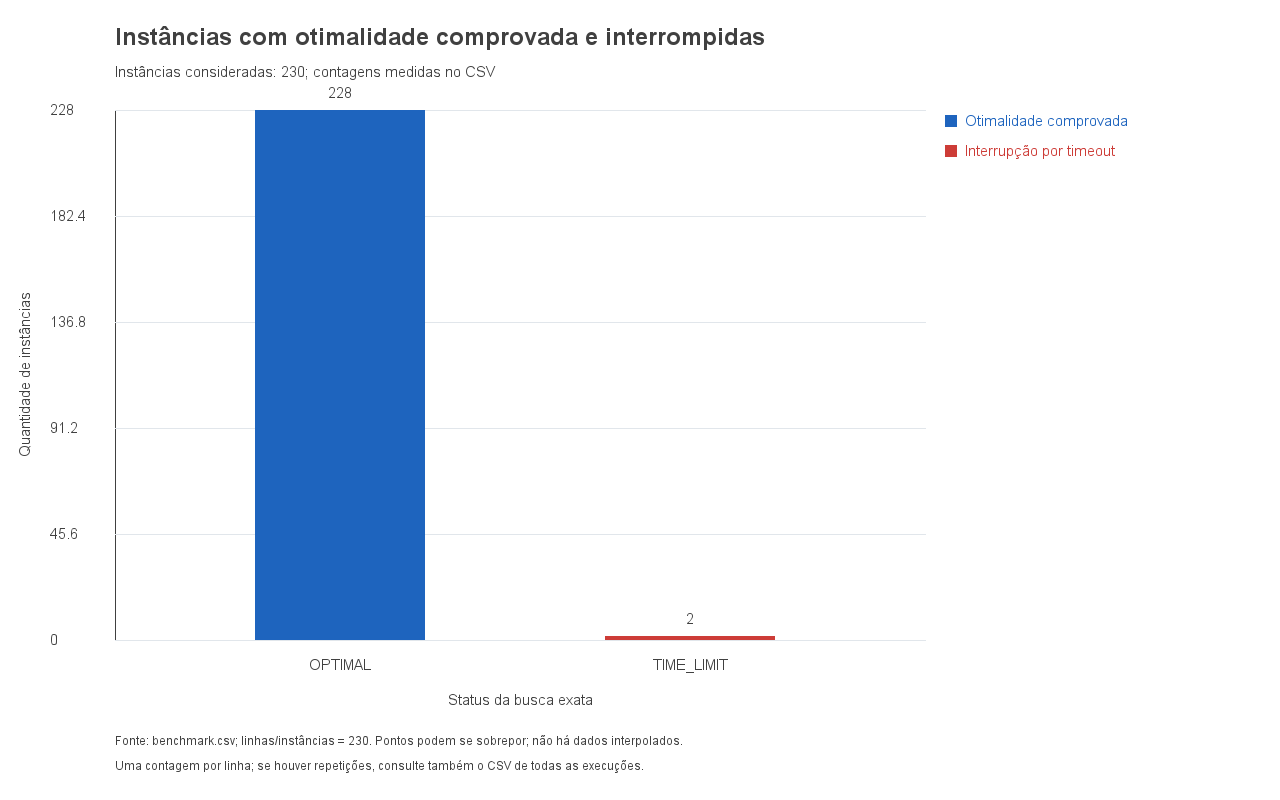
\includegraphics[width=\textwidth]{06-status.png}
\caption{Conclusão da busca exata nas 230 instâncias: 228 provas de ótimo e dois timeouts na execução selecionada de cada grafo. Fonte: benchmark original.}
\label{fig:status}
\end{figure}
\FloatBarrier

\subsection{Tempos por tamanho e densidade}

A Tabela~\ref{tab:configurations} apresenta as 20 configurações
aleatórias. A dispersão $[Q_1;Q_3]$ é calculada entre as dez
instâncias de cada par $(n,p)$, após a seleção das três medições
de cada algoritmo. As unidades diferentes são explícitas:
milissegundos para o exato e microssegundos para a aproximação.
O único timeout aleatório permanece como observação parcial.

% Gerado dos CSVs reais por ReportStats.java.
\begin{table}[htbp]
\centering
\caption{Tempos nos 200 grafos aleatórios: dez instâncias por configuração. Valores são medianas superiores entre instâncias, seguidas de $[Q_1;Q_3]$. A unidade do exato é ms e a da aproximação é $\mu$s. O tempo parcial do único timeout aleatório foi mantido; O/T conta ótimo/timeout.}
\label{tab:configurations}
\small
\setlength{\tabcolsep}{3pt}
\begin{tabular}{rrrrrl}
\toprule
$n$ & $p$ & $\bar d$ & Exato (ms) & Aprox. ($\mu$s) & O/T \\
\midrule
10 & 0,1 & 0,100 & 0,025 [0,022;0,028] & 5,70 [4,90;6,10] & 10/0 \\
10 & 0,3 & 0,289 & 0,039 [0,033;0,045] & 6,40 [5,80;6,60] & 10/0 \\
10 & 0,5 & 0,491 & 0,062 [0,047;0,097] & 3,20 [2,60;4,30] & 10/0 \\
10 & 0,7 & 0,729 & 0,067 [0,057;0,075] & 2,50 [2,20;2,80] & 10/0 \\
15 & 0,1 & 0,088 & 0,027 [0,015;0,036] & 1,40 [1,20;1,50] & 10/0 \\
15 & 0,3 & 0,276 & 0,102 [0,061;0,115] & 2,30 [2,00;2,60] & 10/0 \\
15 & 0,5 & 0,485 & 0,441 [0,258;0,485] & 3,30 [2,60;3,80] & 10/0 \\
15 & 0,7 & 0,677 & 1,251 [0,721;1,491] & 4,40 [2,90;5,20] & 10/0 \\
20 & 0,1 & 0,096 & 0,025 [0,017;0,028] & 1,70 [1,50;2,00] & 10/0 \\
20 & 0,3 & 0,289 & 0,482 [0,366;0,776] & 4,00 [3,50;4,50] & 10/0 \\
20 & 0,5 & 0,499 & 5,951 [2,461;6,214] & 5,10 [4,70;6,20] & 10/0 \\
20 & 0,7 & 0,702 & 6,152 [4,356;14,484] & 1,80 [1,50;2,00] & 10/0 \\
25 & 0,1 & 0,102 & 0,048 [0,033;0,053] & 0,70 [0,40;0,80] & 10/0 \\
25 & 0,3 & 0,293 & 1,992 [0,888;2,317] & 1,20 [1,10;1,70] & 10/0 \\
25 & 0,5 & 0,492 & 17,049 [13,597;19,951] & 1,90 [1,90;2,20] & 10/0 \\
25 & 0,7 & 0,710 & 133,245 [89,431;136,566] & 2,40 [2,10;2,40] & 10/0 \\
30 & 0,1 & 0,103 & 0,054 [0,036;0,157] & 0,70 [0,50;0,90] & 10/0 \\
30 & 0,3 & 0,295 & 22,094 [18,207;54,949] & 2,00 [1,90;2,10] & 10/0 \\
30 & 0,5 & 0,496 & 560,041 [218,852;586,354] & 2,30 [2,20;2,50] & 10/0 \\
30 & 0,7 & 0,685 & 3865,782 [2441,897;4069,889] & 2,60 [2,50;2,80] & 9/1 \\
\bottomrule
\end{tabular}
\end{table}


Para $p=0{,}5$, a mediana superior do exato entre instâncias
passa de 0,062~ms em $n=10$ para 560,041~ms em $n=30$.
Para $n=30$, varia de 0,054~ms em $p=0{,}1$ a
3\,865,782~ms em $p=0{,}7$, com um timeout na última configuração.
Na aproximação, as medianas das 20 configurações ficam entre
0,70 e 6,40~$\mu$s. Esses números são observações da execução,
e sua interpretação requer considerar a ordem da coleta e o
ambiente da JVM.

A Tabela~\ref{tab:sizes} agrega, para cada $n$, os 40 grafos
aleatórios das quatro probabilidades. A mediana de nós explorados
vai de 17 para 536\,777; a de podas, de 7 para 268\,385.
Cada coluna é agregada separadamente, e não representa
necessariamente uma mesma instância do grupo.

% Gerado dos CSVs reais por ReportStats.java.
\begin{table}[htbp]
\centering
\caption{Resumo por tamanho nos grafos aleatórios (40 instâncias por linha, quatro probabilidades). Tempos, nós e podas são medianas superiores entre instâncias. Contagens em timeout são parciais.}
\label{tab:sizes}
\small
\begin{tabular}{rrrrrr}
\toprule
$n$ & Exato (ms) & Aprox. ($\mu$s) & Nós & Podas & O/T \\
\midrule
10 & 0,050 & 4,90 & 17 & 7 & 40/0 \\
15 & 0,132 & 2,60 & 147 & 72 & 40/0 \\
20 & 1,276 & 3,50 & 1\,083 & 539 & 40/0 \\
25 & 7,451 & 1,90 & 27\,801 & 13\,897 & 40/0 \\
30 & 209,381 & 2,20 & 536\,777 & 268\,385 & 39/1 \\
\bottomrule
\end{tabular}
\end{table}


A Figura~\ref{fig:runtime} exibe os tempos das 230 instâncias,
incluindo as estruturadas. A escala logarítmica permite observar
as diferentes ordens de grandeza. As duas cruzes vermelhas são
tempos até interrupção, e não tempos completos para provar o
ótimo. Não há tempos nulos omitidos neste corpus.

\begin{figure}[htbp]
\centering
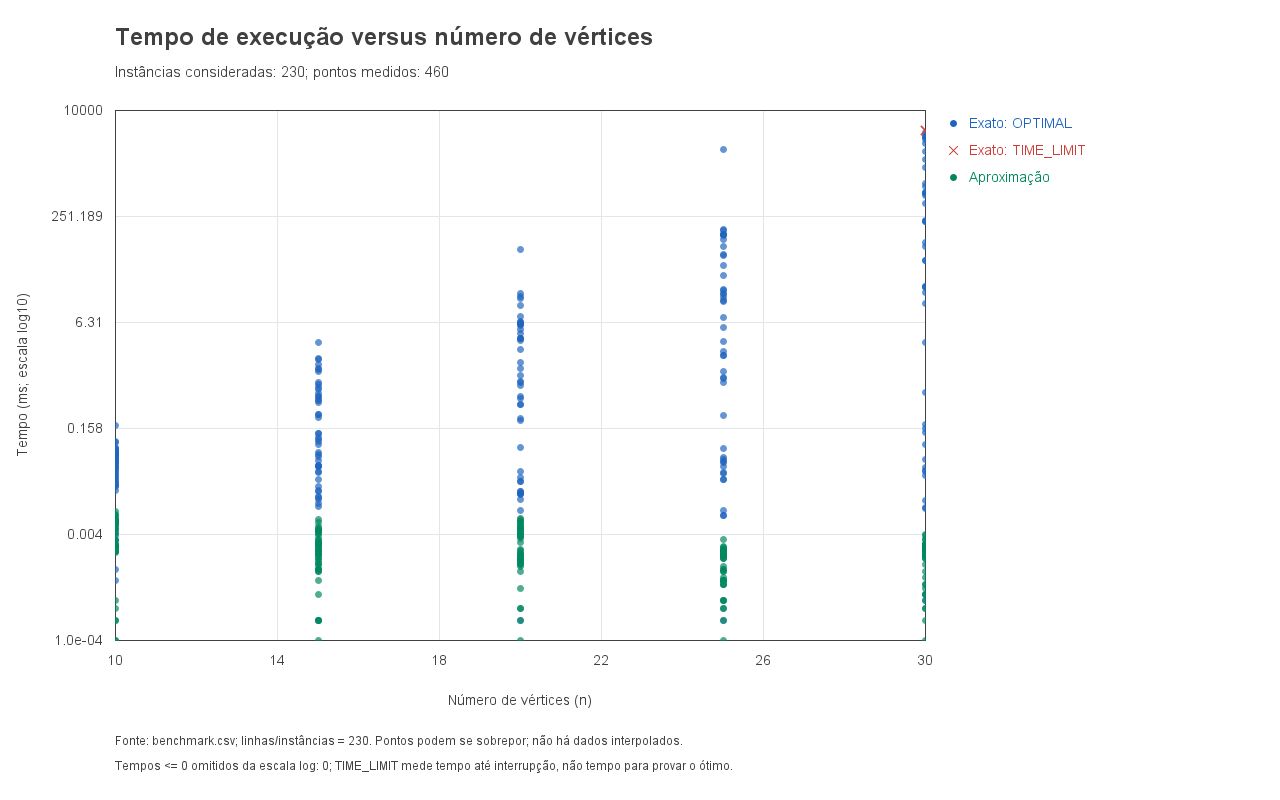
\includegraphics[width=\textwidth]{01-runtime-vs-n.png}
\caption{Tempo versus número de vértices nas 230 instâncias. São 460 pontos medidos, dois por grafo, sujeitos a sobreposição; o eixo vertical usa ms em escala logarítmica. Cruzes indicam timeout.}
\label{fig:runtime}
\end{figure}

A Figura~\ref{fig:density} utiliza a densidade observada da
Equação~\eqref{eq:density}, em vez de $p$. Ela reúne as sete
famílias; portanto, não isola o efeito da densidade do efeito
da estrutura ou de $n$. Para comparar configurações aleatórias
com tamanho fixado, deve-se consultar também a
Tabela~\ref{tab:configurations}.

\begin{figure}[htbp]
\centering
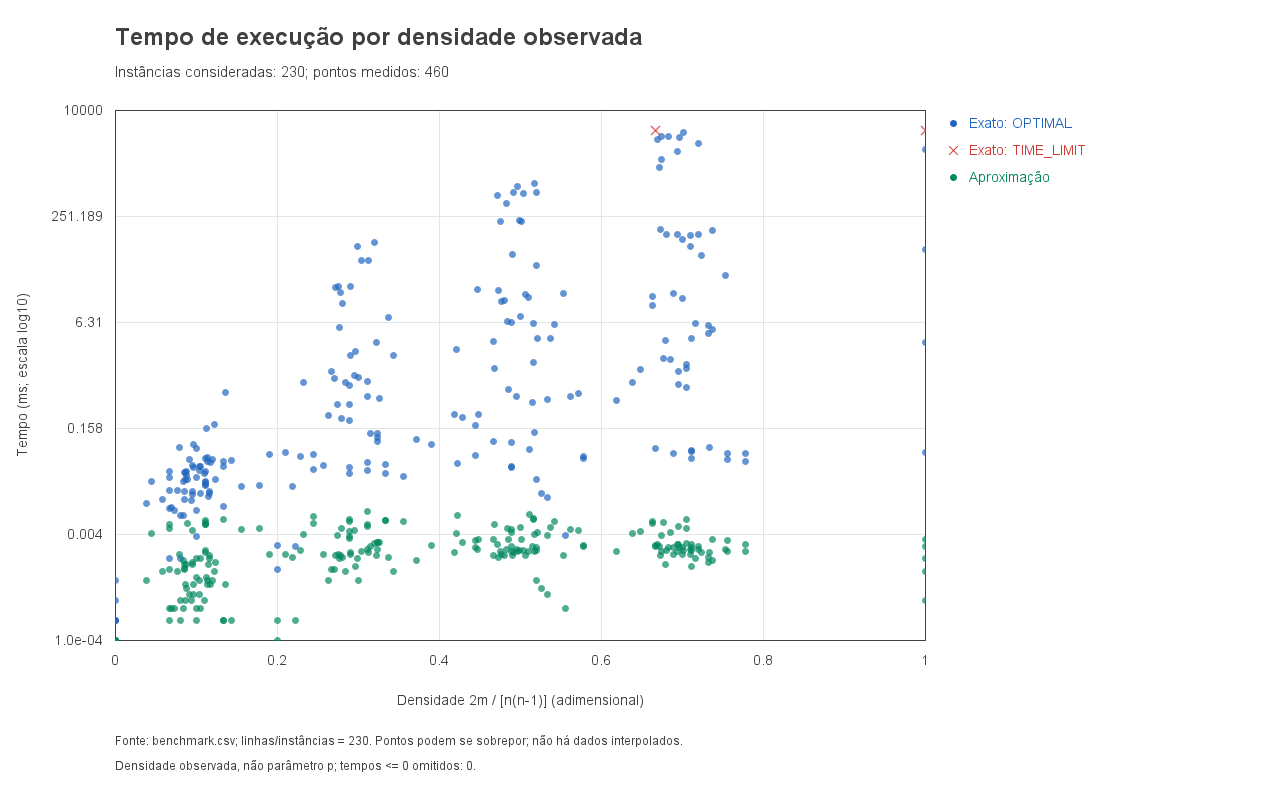
\includegraphics[width=\textwidth]{04-runtime-vs-density.png}
\caption{Tempos em ms por densidade observada: 230 instâncias e 460 pontos. O eixo vertical é logarítmico; valores em timeout são parciais. Famílias e tamanhos diferentes estão reunidos.}
\label{fig:density}
\end{figure}
\FloatBarrier

\subsection{Qualidade das coberturas}

A Tabela~\ref{tab:quality} apresenta as medidas da
Equação~\eqref{eq:quality}, incluindo somente as
\QualityInstances{} instâncias com ótimo comprovado e positivo.
A razão média é \MeanRatio{}, a mediana é \MedianRatio{} e o
gap médio é \MeanGap{}\%. Todas as razões elegíveis pertencem
ao intervalo $[1,2]$. Há \FactorTwoInstances{} casos com razão
exatamente dois. As \ZeroInstances{} instâncias com ótimo zero
retornam cobertura aproximada vazia e não participam dessas
estatísticas; os dois timeouts também são excluídos.

% Gerado dos CSVs reais por ReportStats.java.
\begin{table}[htbp]
\centering
\caption{Qualidade somente com ótimo comprovado e positivo. $\bar R$ é a média das razões individuais, não a razão de médias. Mediana e quartis referem-se a instâncias; gap médio em porcentagem.}
\label{tab:quality}
\small
\setlength{\tabcolsep}{4pt}
\begin{tabular}{lrrrrr}
\toprule
Amostra & $N$ & $\bar R$ & $R_{\mathrm{med}}$ $[Q_1;Q_3]$ & $R_{\max}$ & Gap médio (\%) \\
\midrule
Todas elegíveis & 223 & 1,493 & 1,400 [1,217;1,714] & 2,000 & 49,30 \\
Aleatórias & 199 & 1,453 & 1,385 [1,200;1,636] & 2,000 & 45,31 \\
Estruturadas & 24 & 1,823 & 2,000 [1,846;2,000] & 2,000 & 82,33 \\
\bottomrule
\end{tabular}
\end{table}


Nas instâncias com ótimo positivo, a aproximação coincide
em cardinalidade com o ótimo em \EqualPositiveInstances{} casos:
$K_{15}$ e $K_{25}$. Incluindo os cinco grafos sem arestas,
são \EqualTotalInstances{} coincidências. Isso não muda o
status do algoritmo aproximado para exato.

A Figura~\ref{fig:cover-size} contém as 228 instâncias com
ótimo comprovado, incluindo as cinco de ótimo zero.
As referências $y=x$ e $y=2x$ delimitam a igualdade com
o ótimo e a garantia teórica, respectivamente. A
Figura~\ref{fig:ratio} contém apenas as 223 razões definidas.
Pontos coincidentes não foram deslocados artificialmente.

\begin{figure}[htbp]
\centering
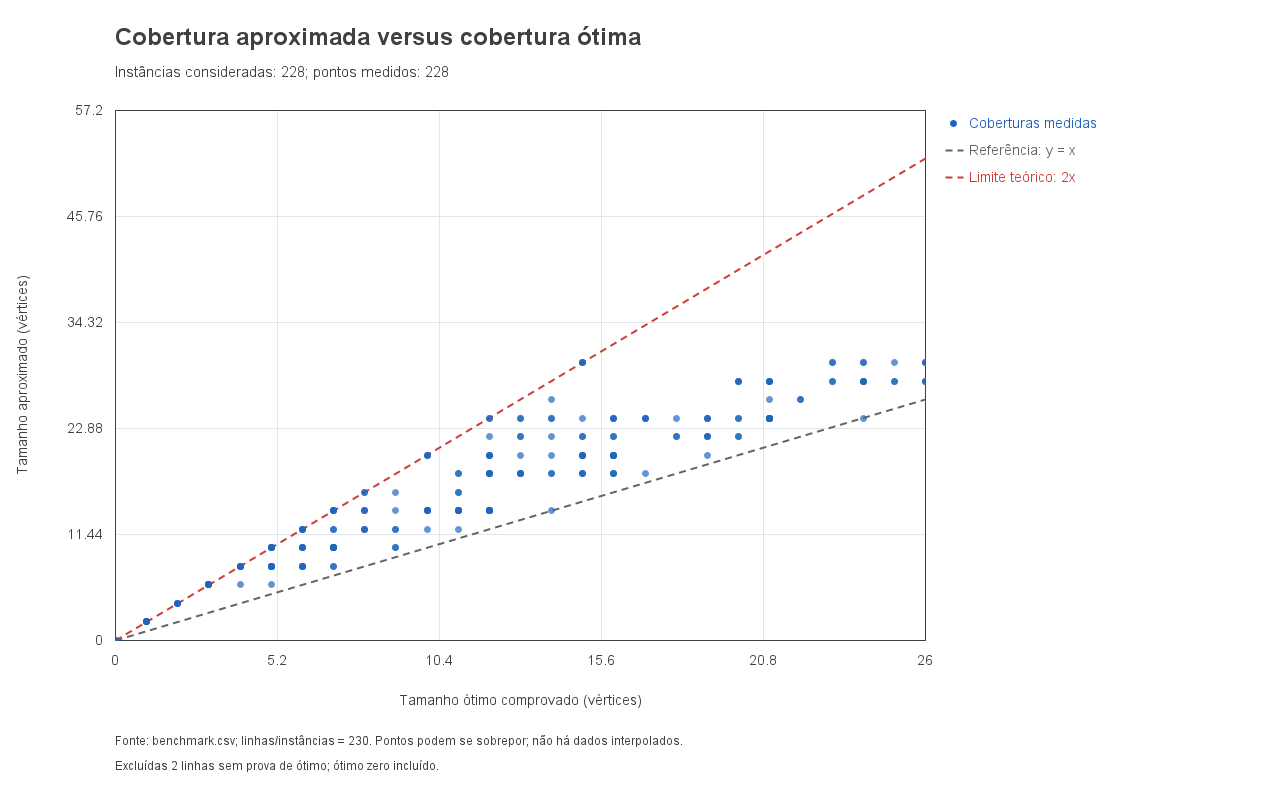
\includegraphics[width=\textwidth]{02-approx-vs-optimum.png}
\caption{Cardinalidade aproximada versus ótima em 228 instâncias com prova. Os dois timeouts são excluídos; ótimos zero são incluídos. Linhas tracejadas são referências teóricas, não medições.}
\label{fig:cover-size}
\end{figure}

\begin{figure}[htbp]
\centering
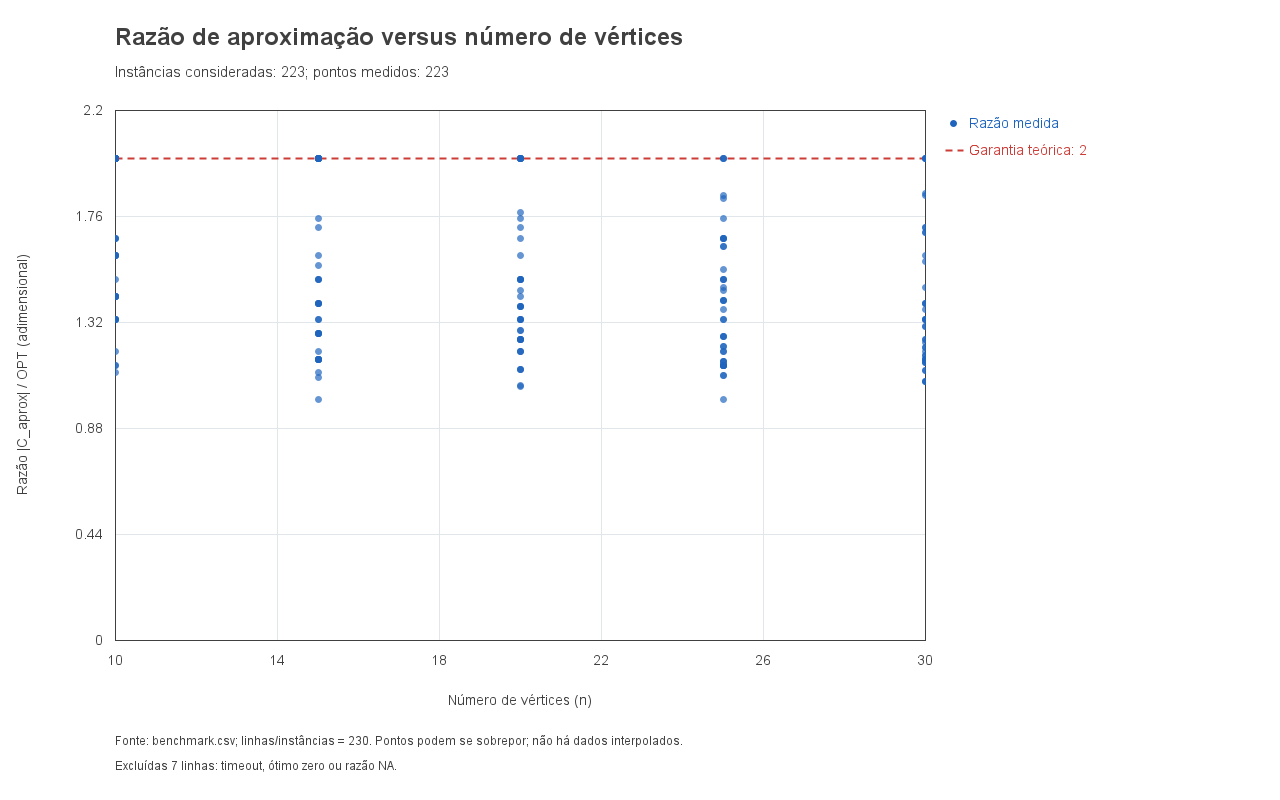
\includegraphics[width=\textwidth]{03-ratio-vs-n.png}
\caption{Razão de aproximação por número de vértices nas 223 instâncias elegíveis. Excluem-se dois timeouts e cinco ótimos zero. A linha em $R=2$ representa a garantia teórica.}
\label{fig:ratio}
\end{figure}
\FloatBarrier

\subsection{Famílias estruturadas e esforço de busca}

A Tabela~\ref{tab:structured} apresenta os 30 grafos estruturados.
O Branch and Bound comprova os valores de controle em 29 deles.
Somente $K_{30}$ termina em timeout. Nos caminhos, estrelas
e bipartidos completos deste conjunto, a aproximação utiliza
exatamente o dobro do ótimo. Os ciclos ímpares têm razões menores
que dois, e os completos ilustram coberturas aproximadas
próximas do mínimo, sem que isso torne simples a certificação
pela busca implementada.

% Gerado dos CSVs reais por ReportStats.java.
\begin{table}[htbp]
\centering
\caption{Resultados das 30 instâncias estruturadas (três medições por algoritmo; linha da mediana). Melhor é a incumbente exata; OPT é preenchido somente com prova. Tempos do exato em ms; nós são estados explorados.}
\label{tab:structured}
\small
\setlength{\tabcolsep}{4pt}
\begin{tabular}{lrrrrrr}
\toprule
Família & $n$ & Melhor & OPT & Aprox. & Exato (ms) & Nós \\
\midrule
Caminho & 10 & 5 & 5 & 10 & 0,0027 & 11 \\
Ciclo & 10 & 5 & 5 & 10 & 0,0026 & 11 \\
Estrela & 10 & 1 & 1 & 2 & 0,0012 & 3 \\
Completo & 10 & 9 & 9 & 10 & 0,0680 & 513 \\
Bipartido completo & 10 & 5 & 5 & 10 & 0,0039 & 11 \\
Sem arestas & 10 & 0 & 0 & 0 & 0,0008 & 0 \\
Caminho & 15 & 7 & 7 & 14 & 0,0425 & 15 \\
Ciclo & 15 & 8 & 8 & 14 & 0,0525 & 17 \\
Estrela & 15 & 1 & 1 & 2 & 0,0106 & 3 \\
Completo & 15 & 14 & 14 & 14 & 3,1101 & 16\,383 \\
Bipartido completo & 15 & 7 & 7 & 14 & 0,0144 & 15 \\
Sem arestas & 15 & 0 & 0 & 0 & 0,0002 & 0 \\
Caminho & 20 & 10 & 10 & 20 & 0,0093 & 21 \\
Ciclo & 20 & 10 & 10 & 20 & 0,0167 & 21 \\
Estrela & 20 & 1 & 1 & 2 & 0,0037 & 3 \\
Completo & 20 & 19 & 19 & 20 & 81,0001 & 524\,289 \\
Bipartido completo & 20 & 10 & 10 & 20 & 0,0168 & 21 \\
Sem arestas & 20 & 0 & 0 & 0 & 0,0002 & 0 \\
Caminho & 25 & 12 & 12 & 24 & 0,0077 & 25 \\
Ciclo & 25 & 13 & 13 & 24 & 0,0078 & 27 \\
Estrela & 25 & 1 & 1 & 2 & 0,0017 & 3 \\
Completo & 25 & 24 & 24 & 24 & 2621,2069 & 16\,777\,215 \\
Bipartido completo & 25 & 12 & 12 & 24 & 0,0268 & 25 \\
Sem arestas & 25 & 0 & 0 & 0 & 0,0002 & 0 \\
Caminho & 30 & 15 & 15 & 30 & 0,0099 & 31 \\
Ciclo & 30 & 15 & 15 & 30 & 0,0100 & 31 \\
Estrela & 30 & 1 & 1 & 2 & 0,0017 & 3 \\
Completo & 30 & 29 & NA & 30 & 5000,0004$^{*}$ & 31\,109\,928 \\
Bipartido completo & 30 & 15 & 15 & 30 & 0,1362 & 31 \\
Sem arestas & 30 & 0 & 0 & 0 & 0,0004 & 0 \\
\bottomrule
\end{tabular}

\smallskip
{\footnotesize $^{*}$TIME\_LIMIT: tempo e nós parciais; sem certificado de ótimo.}
\end{table}


A Figura~\ref{fig:nodes} apresenta todos os grafos, com
$\text{nós}+1$ no eixo vertical logarítmico para representar
também o caso zero. Grafos sem arestas não exigem estados
de busca. Em $K_{20}$ e $K_{25}$, os estados explorados são
524\,289 e 16\,777\,215, respectivamente; a razão entre
essas contagens é próxima de 32 para cinco vértices adicionais.
Em contraste, o bipartido completo com 30 vértices é resolvido
com 31 estados. São diferenças de estrutura, não apenas de tamanho.

\begin{figure}[htbp]
\centering
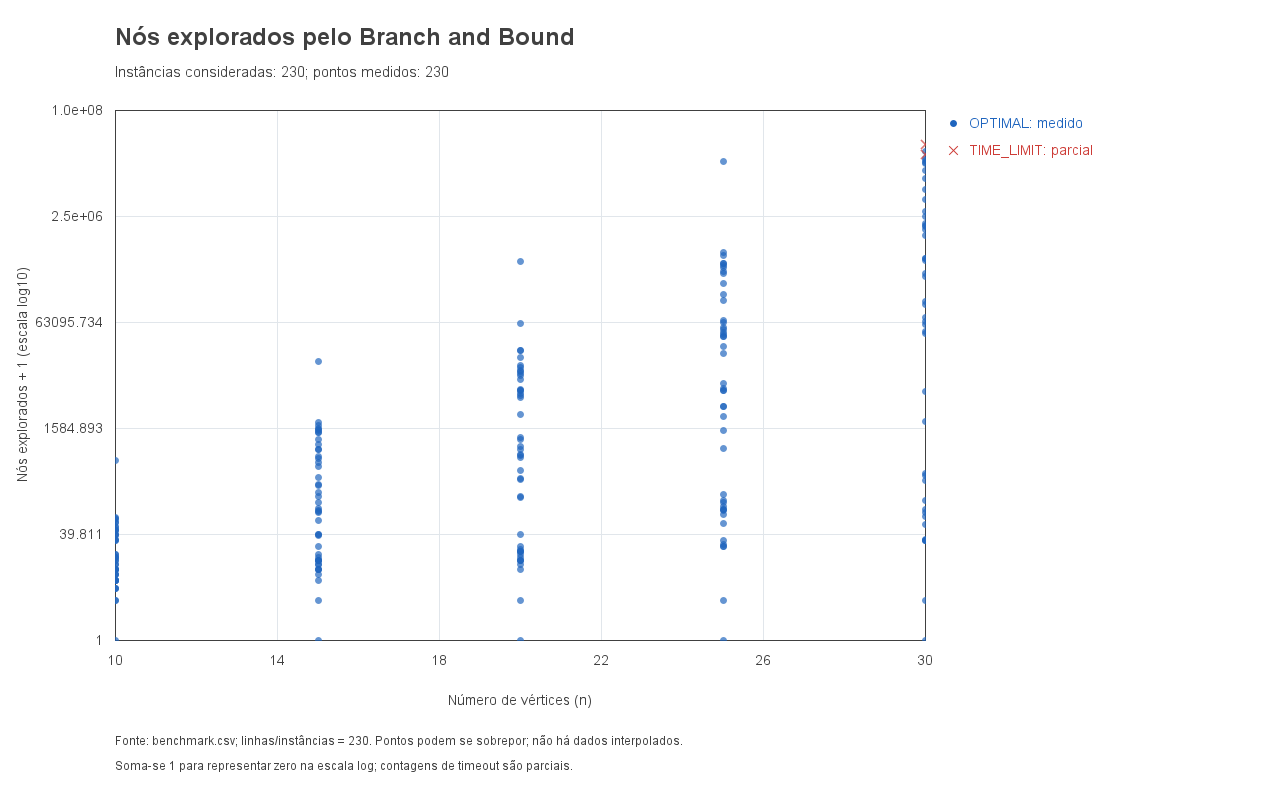
\includegraphics[width=\textwidth]{05-explored-nodes.png}
\caption{Estados explorados pelo Branch and Bound em 230 instâncias. O eixo vertical representa contagem mais um em escala logarítmica; cruzes vermelhas são contagens parciais de timeout.}
\label{fig:nodes}
\end{figure}
\FloatBarrier

\subsection{Instâncias interrompidas}

A Tabela~\ref{tab:timeouts} detalha os timeouts selecionados:
\path{random_n30_p0.7_i06}, com semente 20261311, e
\path{complete_n30}. As melhores coberturas conhecidas têm
tamanhos 26 e 29, enquanto a aproximação tem tamanhos 28 e 30.
Nenhuma razão ou gap é calculado a partir desses pares.

% Gerado dos CSVs reais por ReportStats.java.
\begin{table}[htbp]
\centering
\caption{As duas instâncias com TIME\_LIMIT no resumo. Tempos em ms e contagens pertencem às execuções selecionadas; ótimo, razão e gap são NA em ambas. Cada instância teve três timeouts nas medições individuais.}
\label{tab:timeouts}
\small
\setlength{\tabcolsep}{4pt}
\begin{tabular}{lrrrrr}
\toprule
Instância & Melhor & Aprox. & Tempo parcial & Nós & Podas \\
\midrule
$G(30;0{,}7)$, $i=6$ & 26 & 28 & 5000,0605 & 21\,986\,165 & 10\,993\,076 \\
$K_{30}$ & 29 & 30 & 5000,0004 & 31\,109\,928 & 15\,554\,955 \\
\bottomrule
\end{tabular}
\end{table}


As três medições de cada uma das duas instâncias foram
interrompidas, explicando os seis timeouts individuais.
O pequeno excesso em relação a 5\,000~ms é compatível com o
controle cooperativo do código. O registro global de
146,665~s inclui validação, exportação e progresso, não
sendo um tempo individual nem uma soma exclusiva das
chamadas dos algoritmos.
\FloatBarrier

\section{Análise dos Resultados}
\label{sec:analysis}

\subsection{Tempo, escalabilidade e estrutura}

\textbf{Resultado observado.}
A aproximação tem tempo menor nas \FasterApproxInstances{} de
\TotalInstances{} comparações de execuções selecionadas, incluindo
os grafos sem arestas. No exato, as medianas dos grupos aleatórios
crescem com $n$ na Tabela~\ref{tab:sizes}. Para $p=0{,}5$,
a diferença entre os extremos da grade é de várias ordens de
grandeza, enquanto a aproximação permanece na escala de
microssegundos.

\textbf{Explicação possível.}
A aproximação faz uma passagem pelas arestas e usa marcações
por vértice. O exato, além do custo de sua incumbente inicial,
recalcula graus e limites em numerosos estados e copia conjuntos
de bits. A ampliação da árvore de busca observada é coerente
com o comportamento exponencial possível dessa estratégia.
Não se trata de uma demonstração experimental da notação
assintótica: a justificativa de complexidade é algorítmica.

\textbf{Limitação.}
Os tempos aproximados não crescem monotonicamente com $n$.
Por exemplo, a mediana agregada é 4,90~$\mu$s para $n=10$
e 2,20~$\mu$s para $n=30$. Esse resultado não indica que o
algoritmo se torna assintoticamente mais rápido. A coleta usa
uma única JVM, instâncias em ordem fixa e grafos pequenos;
otimização progressiva pelo compilador em tempo de execução,
resolução do relógio, frequência da CPU e coleta de lixo
podem afetar tempos tão curtos. O aquecimento reduz, mas
não elimina esses fatores. Não houve múltiplas inicializações
independentes da JVM nem cálculo de significância estatística.

Na Tabela~\ref{tab:configurations}, aumentar $p$ com $n$ fixado
está associado a maior tempo mediano do exato em todos os
cinco tamanhos desta grade. A Figura~\ref{fig:density}, porém,
não autoriza concluir que densidade sozinha determina a
dificuldade. O bipartido completo com 30 vértices tem
densidade aproximadamente 0,517 e tempo exato de 0,1362~ms,
enquanto os aleatórios de $n=30,p=0{,}5$, de densidade média
0,496, têm mediana de 560,041~ms. O arranjo das arestas e a
qualidade dos limites também importam.

\subsection{Otimalidade, limites e timeout}

Os 228 resultados \texttt{OPTIMAL} indicam prova produzida pelo
solver; os dois \texttt{TIME\_LIMIT} indicam apenas incumbentes
válidas. Essa distinção é necessária mesmo em uma família
com ótimo teórico conhecido. Em $K_{30}$, o tamanho 29
coincide com a fórmula $n-1$, mas o algoritmo interrompido
não concluiu sua própria certificação. O resultado continua
classificado como timeout, e seus campos de ótimo, razão e
gap permanecem \texttt{NA}.

Uma explicação para o custo dos completos está na força do
limite inferior. Em um completo residual com $r$ vértices,
um matching tem $\lfloor r/2\rfloor$ arestas, enquanto o
mínimo residual é $r-1$. O limite pode, portanto, ficar
distante da quantidade realmente necessária, retardando
podas. Já uma primeira cobertura de boa qualidade e limites
mais próximos do mínimo favorecem outros grafos.
A implementação não utiliza reconhecimento de completos,
algoritmos especializados para bipartidos ou memorização
de subproblemas residuais repetidos.

As contagens de nós e podas sustentam a descrição do esforço
da busca, mas não medem isoladamente o benefício de cada
heurística. Não foram executadas versões sem limite
inferior, sem ordenação por grau ou sem incumbente
aproximada. Assim, atribuir uma aceleração quantitativa
a uma dessas técnicas exigiria uma comparação adicional.
Além disso, os nós e tempos de timeout são observações
censuradas: não permitem estimar quantos estados ou quanto
tempo faltava para concluir a prova.

\subsection{Qualidade e compromisso entre os algoritmos}

A aproximação respeita a garantia de fator~2 em todas as
223 instâncias em que a razão pode ser avaliada.
Seu fator médio de \MeanRatio{} corresponde ao gap médio
de \MeanGap{}\%, e \FactorTwoInstances{} instâncias atingem
exatamente o limite de fator~2. Caminhos, estrelas e
bipartidos completos da suíte tornam visível que a garantia
não é apenas um limite folgado sem ocorrência prática
nesses dados.

As coincidências com o ótimo em $K_{15}$ e $K_{25}$
decorrem da cardinalidade dos extremos emparelhados nesses
completos ímpares: o método deixa um vértice livre e
seleciona $n-1$. São resultados particulares, não uma
capacidade geral de reconhecer quando a solução é ótima.
Nos grafos sem arestas, a coincidência é trivial e deve
ser separada da análise de razão.

A composição da amostra também influencia a média:
o subconjunto aleatório elegível tem média
\RandomMeanRatio{}, enquanto o estruturado elegível tem
\StructuredMeanRatio{} (Tabela~\ref{tab:quality}).
Essa diferença decorre das famílias e sementes escolhidas,
e não demonstra superioridade estatística em uma população
de grafos reais. Os dois timeouts não participam das
estatísticas de qualidade; usar suas incumbentes como
denominador produziria uma razão sem a interpretação
de distância ao ótimo requerida.

O Branch and Bound oferece a vantagem do certificado
quando conclui, ao custo de tempo potencialmente elevado.
O matching maximal oferece execução curta e uma garantia
a priori, mas pode selecionar mais vértices. A escolha
adequada depende de se exigir mínimo comprovado ou de
se aceitar uma solução limitada pelo fator~2. A amostra,
restrita a grafos sintéticos de até 30 vértices e a uma
máquina, não sustenta superioridade universal, extrapolação
para redes maiores ou conclusões sobre modelos ponderados.

\section{Conclusão}
\label{sec:conclusion}

Este trabalho formalizou o Problema da Cobertura Mínima
por Vértices, apresentou a NP-Completude de sua versão
de decisão e comparou duas implementações em Java~17
puro: Branch and Bound e matching maximal
2-aproximado. Os testes independentes, os controles
estruturados e a preservação de sementes e medições
permitiram relacionar fundamentos e comportamento
experimental de maneira auditável.

Na execução analisada, o exato comprovou
\OptimalInstances{} ótimos entre \TotalInstances{}
instâncias e foi interrompido em duas; as três repetições
dessas instâncias explicam os seis timeouts individuais.
A aproximação apresentou menor tempo em todas as
comparações selecionadas. Nas \QualityInstances{}
instâncias com ótimo positivo comprovado, sua razão
média foi \MeanRatio{}, sem violação do limite~2.
Esse ganho de tempo veio acompanhado de coberturas
eventualmente maiores, enquanto a certificação do mínimo
impôs custos elevados ao exato em parte dos grafos.

Os objetivos foram atendidos no escopo da implementação
e do corpus utilizado, sem converter incumbentes após
timeout em ótimos comprovados. Permanecem limitações
de escala, de diversidade das instâncias e de controle
da JVM. Como trabalhos futuros, propõem-se melhores
incumbentes iniciais, limites inferiores mais fortes,
redução ou memorização de subproblemas, avaliação
separada das heurísticas, outras aproximações e estudo
de grafos reais. Múltiplas execuções independentes da
JVM e parametrizações pelo tamanho da cobertura
também permitiriam aprofundar a análise.


\FloatBarrier
\bibliographystyle{sbc}
\bibliography{references}

\clearpage
\appendix
\section{Anexos: código-fonte}
\label{app:source}

As Listagens~\ref{lst:edge}--\ref{lst:benchmark} apresentam
integralmente os arquivos centrais da implementação auditada.
Eles foram copiados sem edição; a numeração corresponde às
linhas de cada arquivo. O destaque tipográfico e a quebra
visual de linhas são feitos pelo pacote \texttt{listings},
sem alterar os fontes.

O pacote eletrônico inclui, em \path{codigo/src/}, todos
os arquivos da aplicação, inclusive leitura/exportação,
gráficos, relatório e interface. Em \path{codigo/tests/}
está o \texttt{TestRunner.java} completo. A
Listagem~\ref{lst:tests} reproduz um trecho explicitamente
delimitado desse teste, com o oráculo independente e as
verificações de timeout. Assim, os anexos não são
substituídos por um link externo.

\subsection{Modelo e resultados}

\lstinputlisting[caption={Edge.java: validação e normalização da aresta.},label={lst:edge}]{codigo/src/Edge.java}
\lstinputlisting[caption={Graph.java: representação, adjacência, densidade e validação da cobertura.},label={lst:graph}]{codigo/src/Graph.java}
\lstinputlisting[caption={VertexCoverSolution.java: cobertura com cópias defensivas.},label={lst:solution}]{codigo/src/VertexCoverSolution.java}
\lstinputlisting[caption={SolverResult.java: status, tempo, contadores e indicação de prova.},label={lst:result}]{codigo/src/SolverResult.java}

\subsection{Algoritmos}

\lstinputlisting[caption={ExactBranchAndBound.java: busca exata, limites, ordenação e timeout.},label={lst:exact}]{codigo/src/ExactBranchAndBound.java}
\lstinputlisting[caption={MatchingTwoApproximation.java: emparelhamento maximal e cobertura 2-aproximada.},label={lst:approx}]{codigo/src/MatchingTwoApproximation.java}

\subsection{Geração e benchmark}

\lstinputlisting[caption={GraphGenerator.java: famílias, sementes e manifesto das instâncias.},label={lst:generator}]{codigo/src/GraphGenerator.java}
\lstinputlisting[caption={BenchmarkRunner.java: protocolo, validação, seleção por mediana e exportação.},label={lst:benchmark}]{codigo/src/BenchmarkRunner.java}

\subsection{Trecho dos testes independentes}

As linhas 123--207 do arquivo completo contêm a enumeração dos
grafos de teste, a comparação dos algoritmos, o oráculo por
subconjuntos e os testes de timeout. Os demais testes são
descritos na Seção~\ref{sec:methodology} e estão no arquivo
integral distribuído com o projeto LaTeX.

\lstinputlisting[firstline=123,lastline=207,firstnumber=123,caption={TestRunner.java, trecho: força bruta independente e timeout.},label={lst:tests}]{codigo/tests/TestRunner.java}

\clearpage
\section{Anexo de reprodutibilidade e rastreabilidade}
\label{app:reproducibility}

O projeto LaTeX é autocontido: as entradas das figuras, tabelas,
listagens e bibliografia são locais. \path{dados/benchmark.csv}
e \path{dados/benchmark-runs.csv} são cópias literais dos CSVs
analisados; \path{dados/instancias/} contém os grafos e o
manifesto. Os seis PNGs em \path{figures/} são os originais
do benchmark. Os hashes completos e a auditoria constam de
\path{evidencias/}.

O relatório usa os arquivos \path{sbc-template.sty} e
\path{sbc.bst} sem alterações, obtidos do template SBC
fornecido pelo grupo e identificado na página oficial do
Overleaf.\footnote{\raggedright\url{https://www.overleaf.com/latex/templates/sbc-conferences-template/blbxwjwzdngr}}
O documento preserva papel A4, coluna única, margens,
fonte principal, cabeçalho de autores, legendas,
ausência de numeração de páginas e estilo bibliográfico
do modelo. O material inclui uma cópia do template de
origem para conferência.

\subsection{Reproduzir a aplicação e o protocolo}

Na raiz do projeto Java, os comandos a seguir compilam e
testam a aplicação. A geração usa as mesmas sementes;
uma nova medição pode produzir tempos, timeouts e
incumbentes diferentes, e não deve substituir
silenciosamente os dados auditados.

\begin{lstlisting}[language={},numbers=none,basicstyle=\ttfamily\footnotesize,caption={Compilação e testes usando somente o JDK 17.},label={lst:commands}]
javac -encoding UTF-8 --release 17 -Xlint:all -d out src/*.java tests/*.java
java "-Dfile.encoding=UTF-8" "-Djava.awt.headless=true" -cp out TestRunner
java -cp out Main generate --output data/instances/ --seed 20261115
\end{lstlisting}

O comando completo da medição original é mostrado na
Listagem~\ref{lst:benchmark-command}. Deve ser informado
em uma única linha; as quebras exibidas na listagem são
apenas visuais. Para guardar uma nova execução, escolha
outro caminho de saída.

\begin{lstlisting}[language={},numbers=none,basicstyle=\ttfamily\footnotesize,caption={Configuração do benchmark original, com três medições por algoritmo e instância.},label={lst:benchmark-command}]
java -Xms128m -Xmx512m "-Dfile.encoding=UTF-8" "-Djava.awt.headless=true" -cp out Main benchmark --timeout-ms 5000 --repetitions 3 --warmup 100 --output data/results/benchmark.csv
\end{lstlisting}

Para uso didático, o \path{executar.cmd} da aplicação
compila e abre um menu; seu experimento rápido de
oito grafos não é a amostra deste artigo.
A interface completa mantém os comandos individuais.

\subsection{Reproduzir o pós-processamento e o PDF}

Na raiz deste projeto LaTeX, o utilitário
\path{ferramentas/ReportStats.java} audita os dados e
regenera as tabelas, sem medir tempos novos:

\begin{lstlisting}[language={},numbers=none,basicstyle=\ttfamily\footnotesize,caption={Pós-processamento separado da aplicação experimental.},label={lst:postprocess}]
javac -encoding UTF-8 --release 17 -d build/java codigo/src/*.java codigo/tests/*.java ferramentas/ReportStats.java
java "-Dfile.encoding=UTF-8" "-Djava.awt.headless=true" -cp build/java ReportStats
\end{lstlisting}

O \texttt{main.tex} compila com pdfLaTeX e BibTeX.
No Overleaf, basta importar o ZIP fornecido e selecionar
\path{main.tex} como documento principal, usando
pdfLaTeX. O Java não é necessário para compilar o PDF,
pois as tabelas e figuras já estão incluídas. A
Listagem~\ref{lst:latex-build} mostra a sequência local.

\begin{lstlisting}[language={},numbers=none,basicstyle=\ttfamily\footnotesize,caption={Compilação local do artigo e resolução de referências cruzadas.},label={lst:latex-build}]
pdflatex -interaction=nonstopmode -halt-on-error main.tex
bibtex main
pdflatex -interaction=nonstopmode -halt-on-error main.tex
pdflatex -interaction=nonstopmode -halt-on-error main.tex
\end{lstlisting}

Os nomes completos dos autores constam dos metadados do
PDF e do README; a linha do título utiliza iniciais
intermediárias para manter os três autores em uma linha.
O pacote eletrônico permite conferir os dados e os
fontes independentemente da publicação posterior em um
repositório ou projeto compartilhado.

\end{document}
